\input{../preamble}
\input{../usercommands}

\begin{document}
\vspace*{2cm}

{\centerline{\bf\huge AST2000 Lecture Notes}}

\vspace*{1cm}

\newcommand{\PartName}{2D}
\newcommand{\refproblem}[1]{\PartName.\ref{#1}}


{\centerline{\bf\LARGE Part \PartName}}\vspace*{0.25cm}
{\centerline{\bf\LARGE General Relativity: Orbits}}

\vspace*{1cm}

{\centerline{\underline{\LARGE Questions to ponder before the lecture}}}

\vspace*{1cm}

{\large
\begin{enumerate}
\item Do you think that general relativity will influence the orbits of the planets in the solar system? Why/why not? If yes, how?
\item We know from Newtonian dynamics that there are three possible orbits, elliptic, parabolic and hyperbolic, depending on the total energy of the object. In general relativity, there must be at least one more possibility: that the object is swallowed by a black hole. What kind of criterion would you need to decide whether an object's trajectory will belong to this last class of 'orbit'?
\item If you are inside the horizon, how can you measure velocity? The far away observer cannot make measurements, and there can be no shell observers (they would start falling). How would you define velocity?
\end{enumerate}

\begin{Figure}%[htb]
\centering
%\begin{center}
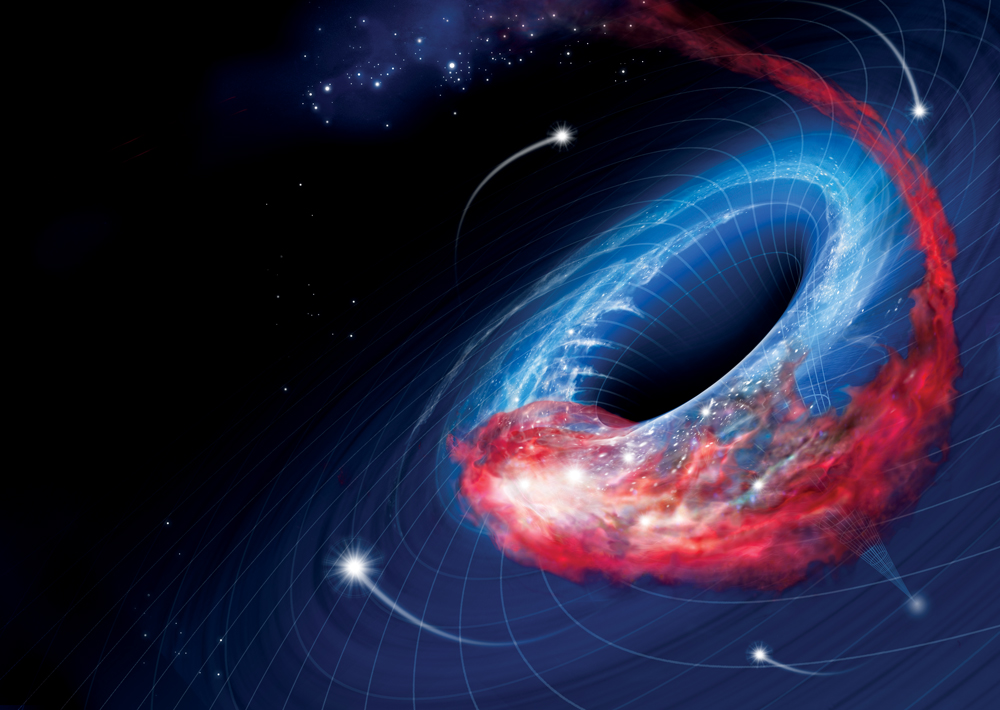
\includegraphics[width=0.8\textwidth]{bh_orbits.jpg}
%\end{center}
\end{Figure}
%Image:Roen Kelly (http://discovermagazine.com/2014/sept/10-to-the-edge-and-back)


\clearpage
\vspace*{2cm}

{\centerline{\bf\huge AST2000 Lecture Notes}}

\vspace*{1cm}
{\centerline{\bf\LARGE Part \PartName}}\vspace*{0.25cm}
{\centerline{\bf\LARGE General Relativity: Orbits}}

\vspace*{1cm}

\begin{multicols}{2}

\section{\ss step-by-step motion}

In this lecture we will look at corrections to orbital motion due to general relativity. We have already learned that a body in the gravitational field of another body may go in elliptical orbits or escape to infinity following parabolic or hyperbolic trajectories depending on the total energy of the body. \textbf{We have now obtained more accurate expressions for motion in gravitational fields and will check if these corrections may give rise to orbital behavior different from the Newtonian prediction} (Hvor har vi fått det?). We will study the motion of a body in the gravitational field of a black hole. We might already anticipate a few differences to Newtonian gravity: If the body comes too close to the black hole (inside the \ss radius), it will be swallowed by the black hole without possibilities to get out. We will now check this in more detail.


\begin{Figure}
\centering
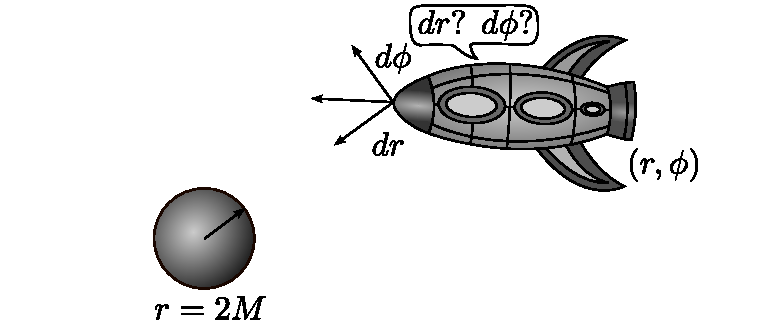
\includegraphics[width=\textwidth]{fig_17-1.pdf}
\captionof{figure}{The spaceship is out of fuel. The engines stop. What will be the next movement in $r$ and $\phi$ direction? \label{fig:stepbystep}}
\end{Figure}

In exercise 2C.4 you deduced some equations of motion for a spaceship in free fall around a black hole. Here we will repeat this exercise. In figure \ref{fig:stepbystep} we show a spaceship at position $(r,\phi,t)$ in \ss coordinates around a black hole of mass $M$. The spaceship has used all its fuel and can therefore not use its engine, it is falling freely. The astronauts in the spaceship are wondering whether the spaceship will pass the black hole so close to the center that they will be swallowed by the black hole or not. We will now study the motion of the spaceship step by step. Do do this we need the new position $(r,\phi,t)$ in \ss coordinates of the spaceship after a time interval $\Delta\tau$ has passed on the wrist watches of the astronauts. Therefore we use small increments in $\Delta r$, $\Delta\phi$ and $\Delta t$ for each small increment in the astronauts proper time $\Delta\tau$. By increasing $\Delta\tau$ and thereby the other coordinates step by step, we will be able to follow the motion $(r,\phi)$ of the spaceship and check if it at some point will reach $r=2M$ or not.

Knowing that the total energy per mass $E/m$ is a constant of motion, we can rewrite the expression
\[
\frac{E}{m}=\sst\frac{dt}{d\tau},
\]
for total energy per mass as
\begin{formbox}
\begin{equation}
\label{eq:t}
\Delta t=\frac{E/m}{\sst}\Delta\tau.
\end{equation}
\end{formbox}
Similarly we can use that the angular momentum per mass $L/m$ is a constant of motion
\[
\frac{L}{m}=r^2\frac{d\phi}{d\tau}
\]
to get\\
\begin{formbox}
\begin{equation}
\label{eq:phi}
\Delta\phi=\frac{L/m}{r^2}\Delta\tau.
\end{equation}
\end{formbox}
We have already obtained the displacements $\Delta\phi$ and $\Delta t$ per proper time interval $\Delta\tau$. Now we need to find the radial displacement $\Delta r$. The \ss line element (see previous lecture) gives
\[
\Delta s^2=\Delta\tau^2=\sst\Delta t^2-\frac{\Delta r^2}{\sst}-r^2\Delta\phi^2.
\]
We insert the expressions (\ref{eq:t}) and (\ref{eq:phi}) into the line element and obtain
\begin{align*}
&\Delta\tau^2=\\
&\sst\left(\frac{E/m}{\sst}\right)^2\Delta\tau^2-\frac{\Delta r^2}{\sst}\\
&-r^2\left(\frac{L/m}{r^2}\right)^2\Delta\tau^2.
\end{align*}
Reorganizing we find
\begin{formbox}
\begin{align}
\label{eq:r}
&\Delta r=\nonumber\\
&\pm\sqrt{\left(\frac{E}{m}\right)^2-\left[1+\left(\frac{L/m}{r}\right)^2\right]\sst}\Delta\tau.
\end{align}
\end{formbox}
We now have three equations (\ref{eq:t}), (\ref{eq:phi}) and (\ref{eq:r}) giving us the motion of the spaceship as observed by the far-away observer for each tick $\Delta\tau$ on the wristwatch of the astronauts. Note that these expressions in reality give the first order terms of a Taylor expansion in $\Delta\tau$. The second derivative terms are not included (and will not be treated in this course) and we can therefore not use them in this form to describe a full orbital motion. 

In the orbital motion, when the radial velocity reaches zero, the spaceship will start moving outwards again (do you see that this is the case? Think about the motion of a planet). Radial velocity equal to zero means that the first derivative is zero and that the second derivatives (second order in the Taylor expansion) is needed in order to describe the next step. But we may use the equations up to the point before the radial velocity equals zero. If the radius at this point is outside $r=2M$ we are saved. If the radial velocity does not reach zero before $r=2M$ the spaceship will fall into the black hole. In order to describe the full motion in a more complete manner we can either continue the Taylor expansion to higher orders or, much easier, we can consider the effective potential.

\section{Effective potential}


\begin{Figure}
\centering
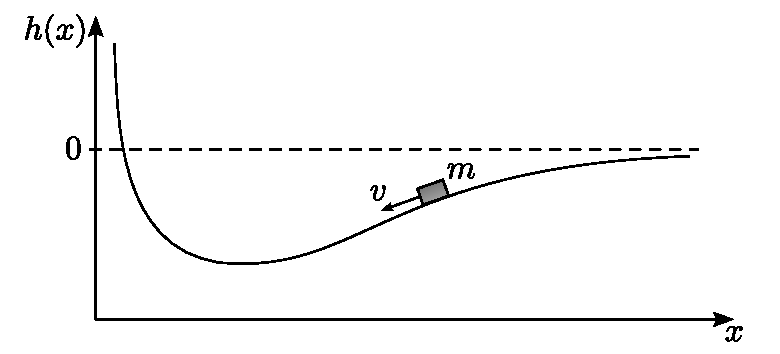
\includegraphics[width=\textwidth]{fig_17-2.pdf}
\captionof{figure}{Object sliding down a frictionless hill with height $h(x)$.\label{fig:fall1}}
\end{Figure}
\begin{Figure}
\centering
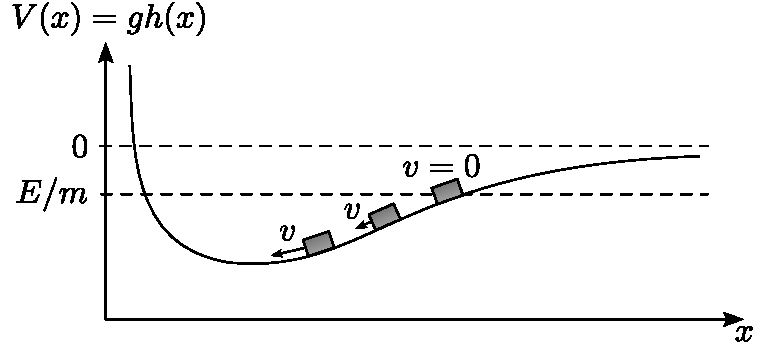
\includegraphics[width=\textwidth]{fig_17-3.pdf}
\captionof{figure}{Object sliding down a frictionless hill with energy per mass $E/m=gh(x)$ deciding the future motion.\label{fig:fall2}}
\end{Figure}



To explain the concept of effective potential, we will go to a well known example: An object sliding down a hill without friction. In figure (\ref{fig:fall1}) we see the situation. An object is located at horizontal position $x$ and at height $h$. We can write the total (Newtonian) energy, kinetic plus potential, with the well known expression
\[
E/m=\frac{1}{2}v^2+gh(x)=\frac{1}{2}v^2+V(x),
\]
where $g$ is the constant gravitational acceleration, $h(x)$ is the height of the hill at position $x$,  $V(x)$ is the potential, $v$ is the velocity of the object and $m$ its mass. In figure \ref{fig:fall2} we see the same plot as figure \ref{fig:fall1}, but the function is now multiplied by $g$ such that the y-axis now shows $gh(x)$ instead of only $h(x)$. Thus, as you see from the previous expression, the units on the y-axis is now energy per mass and the height of the hill is just the potential $V(x)$. When the velocity is zero $v=0$, the height of the object in this plot directly gives us the total $E/m=gh(x)$ for the object (you can see this from the previous equation: if $v=0$ then $E/m=V(x)$). Thus we can draw a horizontal line passing through this point, showing that this is the energy per mass of the object for all positions $x$ (remember that $E/m$ is constant). The object will have velocity zero at all points where the horizontal line intersects the hill curve (why?).

We have defined the height $h(x)$ to go asymptotically to zero for large distances $x\rightarrow\infty$. Thus, at large distances the energy of the object consists of purely kinetic energy as the potential energy $gh(x)\rightarrow0$. A total negative energy of the object corresponds to an object left at rest at $h(x)<0$. This object can never reach infinity: We just learned that at infinity the energy of the object is purely kinetic, but kinetic energy cannot be negative. So an object with a negative total energy is trapped in the 'valley' as seen in the figures. An object with negative energy cannot move all the way in to $x=0$, it can only reach up to the point $E/m$ on the y-axis where the velocity will be zero: It will start oscillating back and forth between the two points where the horizontal line at $E/m$ crosses the hill curve. The situation is different for an object with positive energy: Leave the object far out on the positive x axis with an initial velocity different from zero and so large that $E/m$ is positive. By drawing a horizontal line at $E/m$ you can find how far in the object will move before it has $v=0$ from where it will move back an out to infinity. This object is not bound in the valley. The two situations are illustrated in figure \ref{fig:bound} and \ref{fig:free}.

\begin{Figure}
\centering
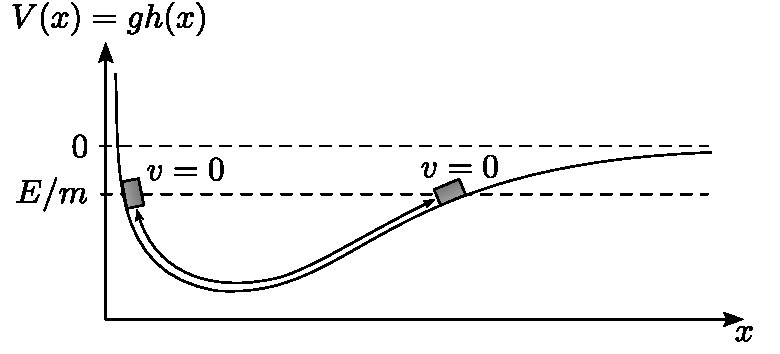
\includegraphics[width=\textwidth]{fig_17-4.pdf}
\captionof{figure}{Bound object oscillating between two points on the hill.\label{fig:bound}}
\end{Figure}
\begin{Figure}
\centering
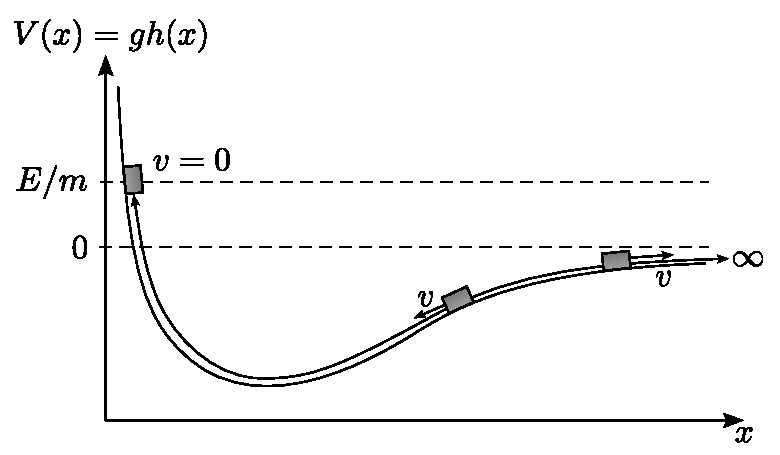
\includegraphics[width=\textwidth]{fig_17-5.pdf}
\captionof{figure}{Free object: slides up to a maximum point and then escapes to infinity.\label{fig:free}}
\end{Figure}


This case was probably not new to you. We will now generalize this situation. We see (from equation \ref{eq:r}) that the equation of motion for this object can be written as
\begin{equation}
\label{eq:general}
A=B\dot{\vec{x}}^2+V(x),
\end{equation}
where $A$ (equal to $E/m$ in our example) and $B$ (equal to $1/2$ in our example) are constants ($B$ being positive), $\vec{x}$ is the position vector of the object and $V(x)$ is the position dependent {\it potential}. If $V(x)$ has a 'valley' similar to figure \ref{fig:fall2} and $V(x)\rightarrow0$ when $x\rightarrow\infty$, then the object with position $\vec{x}$ will move in the following way:
\begin{itemize}
\item With $A<0$ (corresponding to $E<0$ in our example) the object is trapped and will oscillate back and forth between two positions.
\item With $A>0$ (corresponding to $E>0$ in our example), the object can escape out to any position.
\end{itemize}

We recognize the situation described here from a similar physical system: The two body problem. We remember for the two-body problem that an object with negative total energy was bound to orbital motion around the other object whereas objects with positive total energy could escape to infinity. Let's try to see the mathematical analogy. The total energy of an object with mass $m$ close to a star of mass $M$ is
\[
E/m=\frac{1}{2}v^2-G\frac{M}{r},
\] 
and angular momentum
\begin{equation}
\label{eq:spin}
L/m=r^2\dot{\phi}
\end{equation}
using for the moment conventional units. We are only interested in the radial motion of the object, i.e.\ whether the object will be bound or whether it can escape to infinity. We are not interested in the details of the motion in $\phi$ direction. We can rewrite the equation for the energy as
\begin{align}
\label{eq:newton}
&E/m=\frac{1}{2}(\dot{r}^2+r^2\dot{\phi}^2)-G\frac{M}{r}\nonumber\\
&=\frac{1}{2}\dot{r}^2+\left(\frac{1}{2}\frac{(L/m)^2}{r^2}-G\frac{M}{r}\right),
\end{align}
where equation \ref{eq:spin} was used. Setting $A=E/m$, $B=1/2$ and
\begin{formbox}
\[
V_\mathrm{eff}(r)/m=\frac{1}{2}\frac{(L/m)^2}{r^2}-G\frac{M}{r},
\]
\end{formbox}
we see that equation \ref{eq:newton} can be written on the form of equation \ref{eq:general}. We will call the potential $V(r)$ for the {\it effective potential}. Thus the problem is mathematically identical to the problem of the object sliding down the hill. This means that also the results are identical. The $r$ coordinate corresponds to position on the hill, and the effective potential corresponds to the shape of the hill. In figure \ref{fig:newton} we can see the shape of the 'hill' or effective potential. The object falling in the gravitational field of a star is identical to the object sliding down the hill using the effective potential as the shape of the hill. Again we have the result that for $A=E/m<0$, the object is bound and will oscillate between two $r$ positions which we know (from earlier lectures) are $r=a(1-e)$ and $r=a(1+e)$. Here we have ignored the motion in $\phi$ direction, but we already know that this corresponds to an elliptical orbit. For $E/m=0$, the object will reach zero velocity at in infinite distance $r\rightarrow\infty$. We already learned in previous lectures that this corresponds to the parabolic trajectory. Finally for $E/m>0$, the object can move to infinite distances with arbitrary velocity corresponding to the hyperbolic trajectory. Even though the treatment with effective potential did not give us the exact shape of the orbit it did tell us the essentials using the radial motion only: The object can either oscillate between two radial positions or it can move out to infinity depending on the total energy $E/m$.


\begin{Figure}
\centering
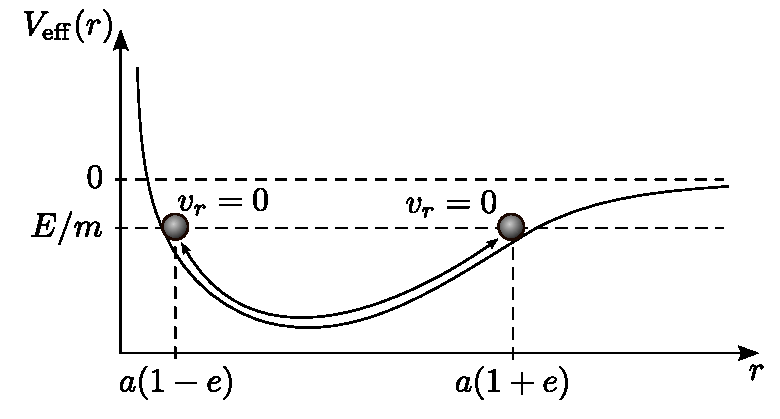
\includegraphics[width=\textwidth]{fig_17-6.pdf}
\captionof{figure}{A bound object in elliptical orbit in a Newtonian effective potential.\label{fig:newton}}
\end{Figure}


\section{Orbital motion in \ss geometry}

We will now turn to the relativistic case. We have seen that by looking just at the radial motion of an object in a gravitational field we can obtain essential information about the future motion of this object without going into details. Equation \ref{eq:r} can be written as
\begin{equation}
\label{eq:rr}
\left(\frac{dr}{d\tau}\right)^2=\left(\frac{E}{m}\right)^2-\left(1-\frac{2M}{r}\right)\left[1+\frac{(L/m)^2}{r^2}\right].
\end{equation}
Again comparing to equation \ref{eq:general} we see that we can make the following substitutions: $A=(E/m)^2$, $B=1$ and
\begin{formbox}
\[
\frac{V_{\rm eff}(r)}{m}=\sqrt{\left(1-\frac{2M}{r}\right)\left[1+\frac{(L/m)^2}{r^2}\right]}
\]
\end{formbox}
We have defined the effective potential such that the square of the effective potential appears in equation \ref{eq:rr}, different from the previous cases. This is just to have an effective potential with units energy. Note that $A$ is now the energy per mass $E/m$ {\it squared} instead of just $E/m$ as we had in the above examples. In the relativistic case we therefore get 
\begin{equation}\label{eq:relativistic_motion}
A=B\dot{\vec{x}}^2+V(x)^2.
\end{equation}
In equation \ref{eq:general} we only required $A$ to be a constant, it is not required that it equals energy. So we still have exactly the same case as we had above and we can use the same argumentation. Note one more difference: The effective potential goes to $V(r)\rightarrow1$ for large distances instead of $V(r)\rightarrow0$ as above (see the plot of the effective potential in figure \ref{fig:rr}). The reason for this is that the rest energy for a particle in relativistic dynamics is $E/m=1$. If the velocity of the object is zero at large distances then $E/m=1$ whereas in Newtonian dynamics $V(r)\rightarrow0$ because $E/m=0$ at large distances. Remember that in Newtonian dynamics we do not consider the rest energy $E=m$. This makes one difference in our argumentation with respect to above. In the Newtonian case, the limiting energy deciding whether the object would be trapped in the potential and therefore stay in a bound orbit or if it would escape to infinity was $E/m=0$. As we see, in relativistic dynamics this limit is $E/m=1$. If $E/m<1$ then the ball starts falling with zero velocity at some point on the hill below $E/m=1$ and it can therefore never escape to $r\rightarrow\infty$, it will start orbiting. If however the energy $E/m>1$ it has the possibility to escape to infinity as it will have a non-zero velocity as $r\rightarrow\infty$ (check that you understand this by looking at equation \ref{eq:rr} and figure \ref{fig:rr}).


\begin{Figure}
\centering
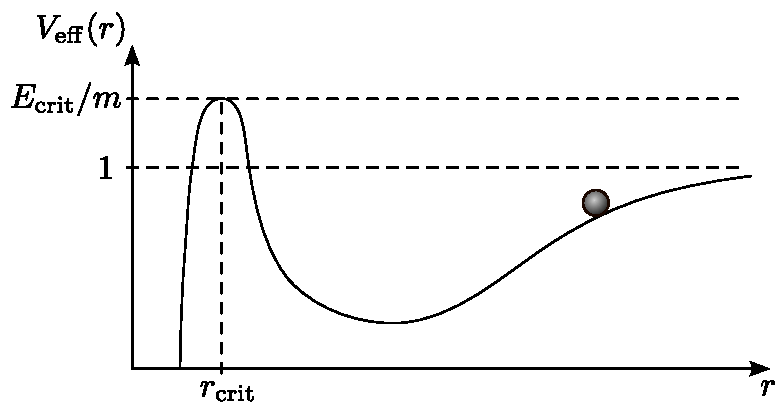
\includegraphics[width=\textwidth]{fig_17-7.pdf}
\captionof{figure}{A bound object in elliptical orbit in a \ss effective potential.\label{fig:rr}}
\end{Figure}

\begin{Figure}
\centering
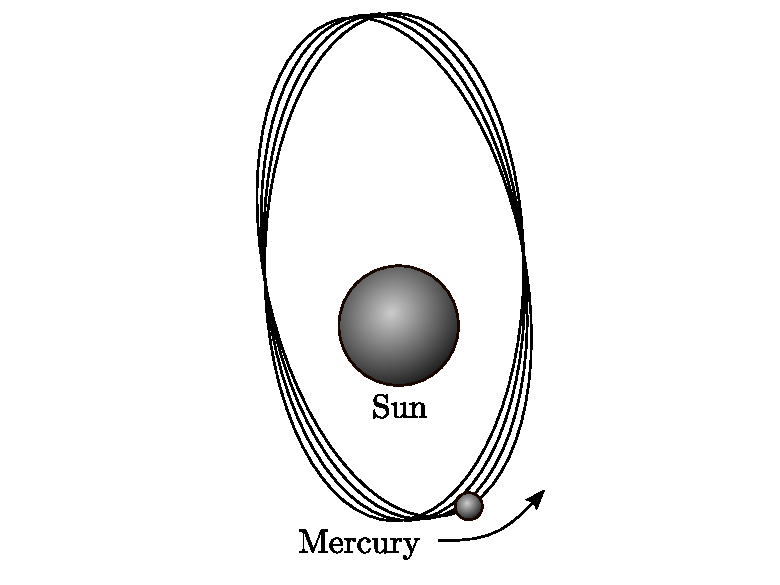
\includegraphics[width=\textwidth]{fig_17-8.pdf}
\captionof{figure}{Perihelion precision of Mercury.\label{fig:peripre}}
\end{Figure}


\begin{figure*}
\fcolorbox{black}{yellow}{\parbox{\dimexpr \linewidth-2\fboxsep-2\fboxrule}{
\begin{minipage}{0.6\textwidth}%{\dimexpr\linewidth-2\fboxsep-2\fboxrule}\parskip=6pt
{\small
\fontfamily{bch}\selectfont
\vspace*{-0.3cm}\hspace*{-0.15cm}\fcolorbox{black}{black}{\bf\color{white} Fact sheet:\color{black}} 
This simulated view based on real data shows stars orbiting the supermassive black hole at the center of the Milky Way along with blue lines marking their orbits. Also, a gas cloud (above center, with its orbit shown in red) has recently been observed approaching the black hole at more than 8 million km/h. The stars and the cloud are shown in their actual positions in 2011. Extremely precise measurements of the stellar orbits in the galactic center show that the supermassive black hole, formally known as Sgr A* (pronounced Sagittarius A star), has a mass of 4.1 million solar masses. The interstellar dust that fills the galaxy blocks our view of the Milky Way's central region in visible light, but astronomers use infrared wavelengths that can penetrate the dust to probe the region.(Figure: ESO)
}
\end{minipage}%\hspace*{0.5cm}
\ \ \ \ \ \ \begin{minipage}{0.35\textwidth}
\centering
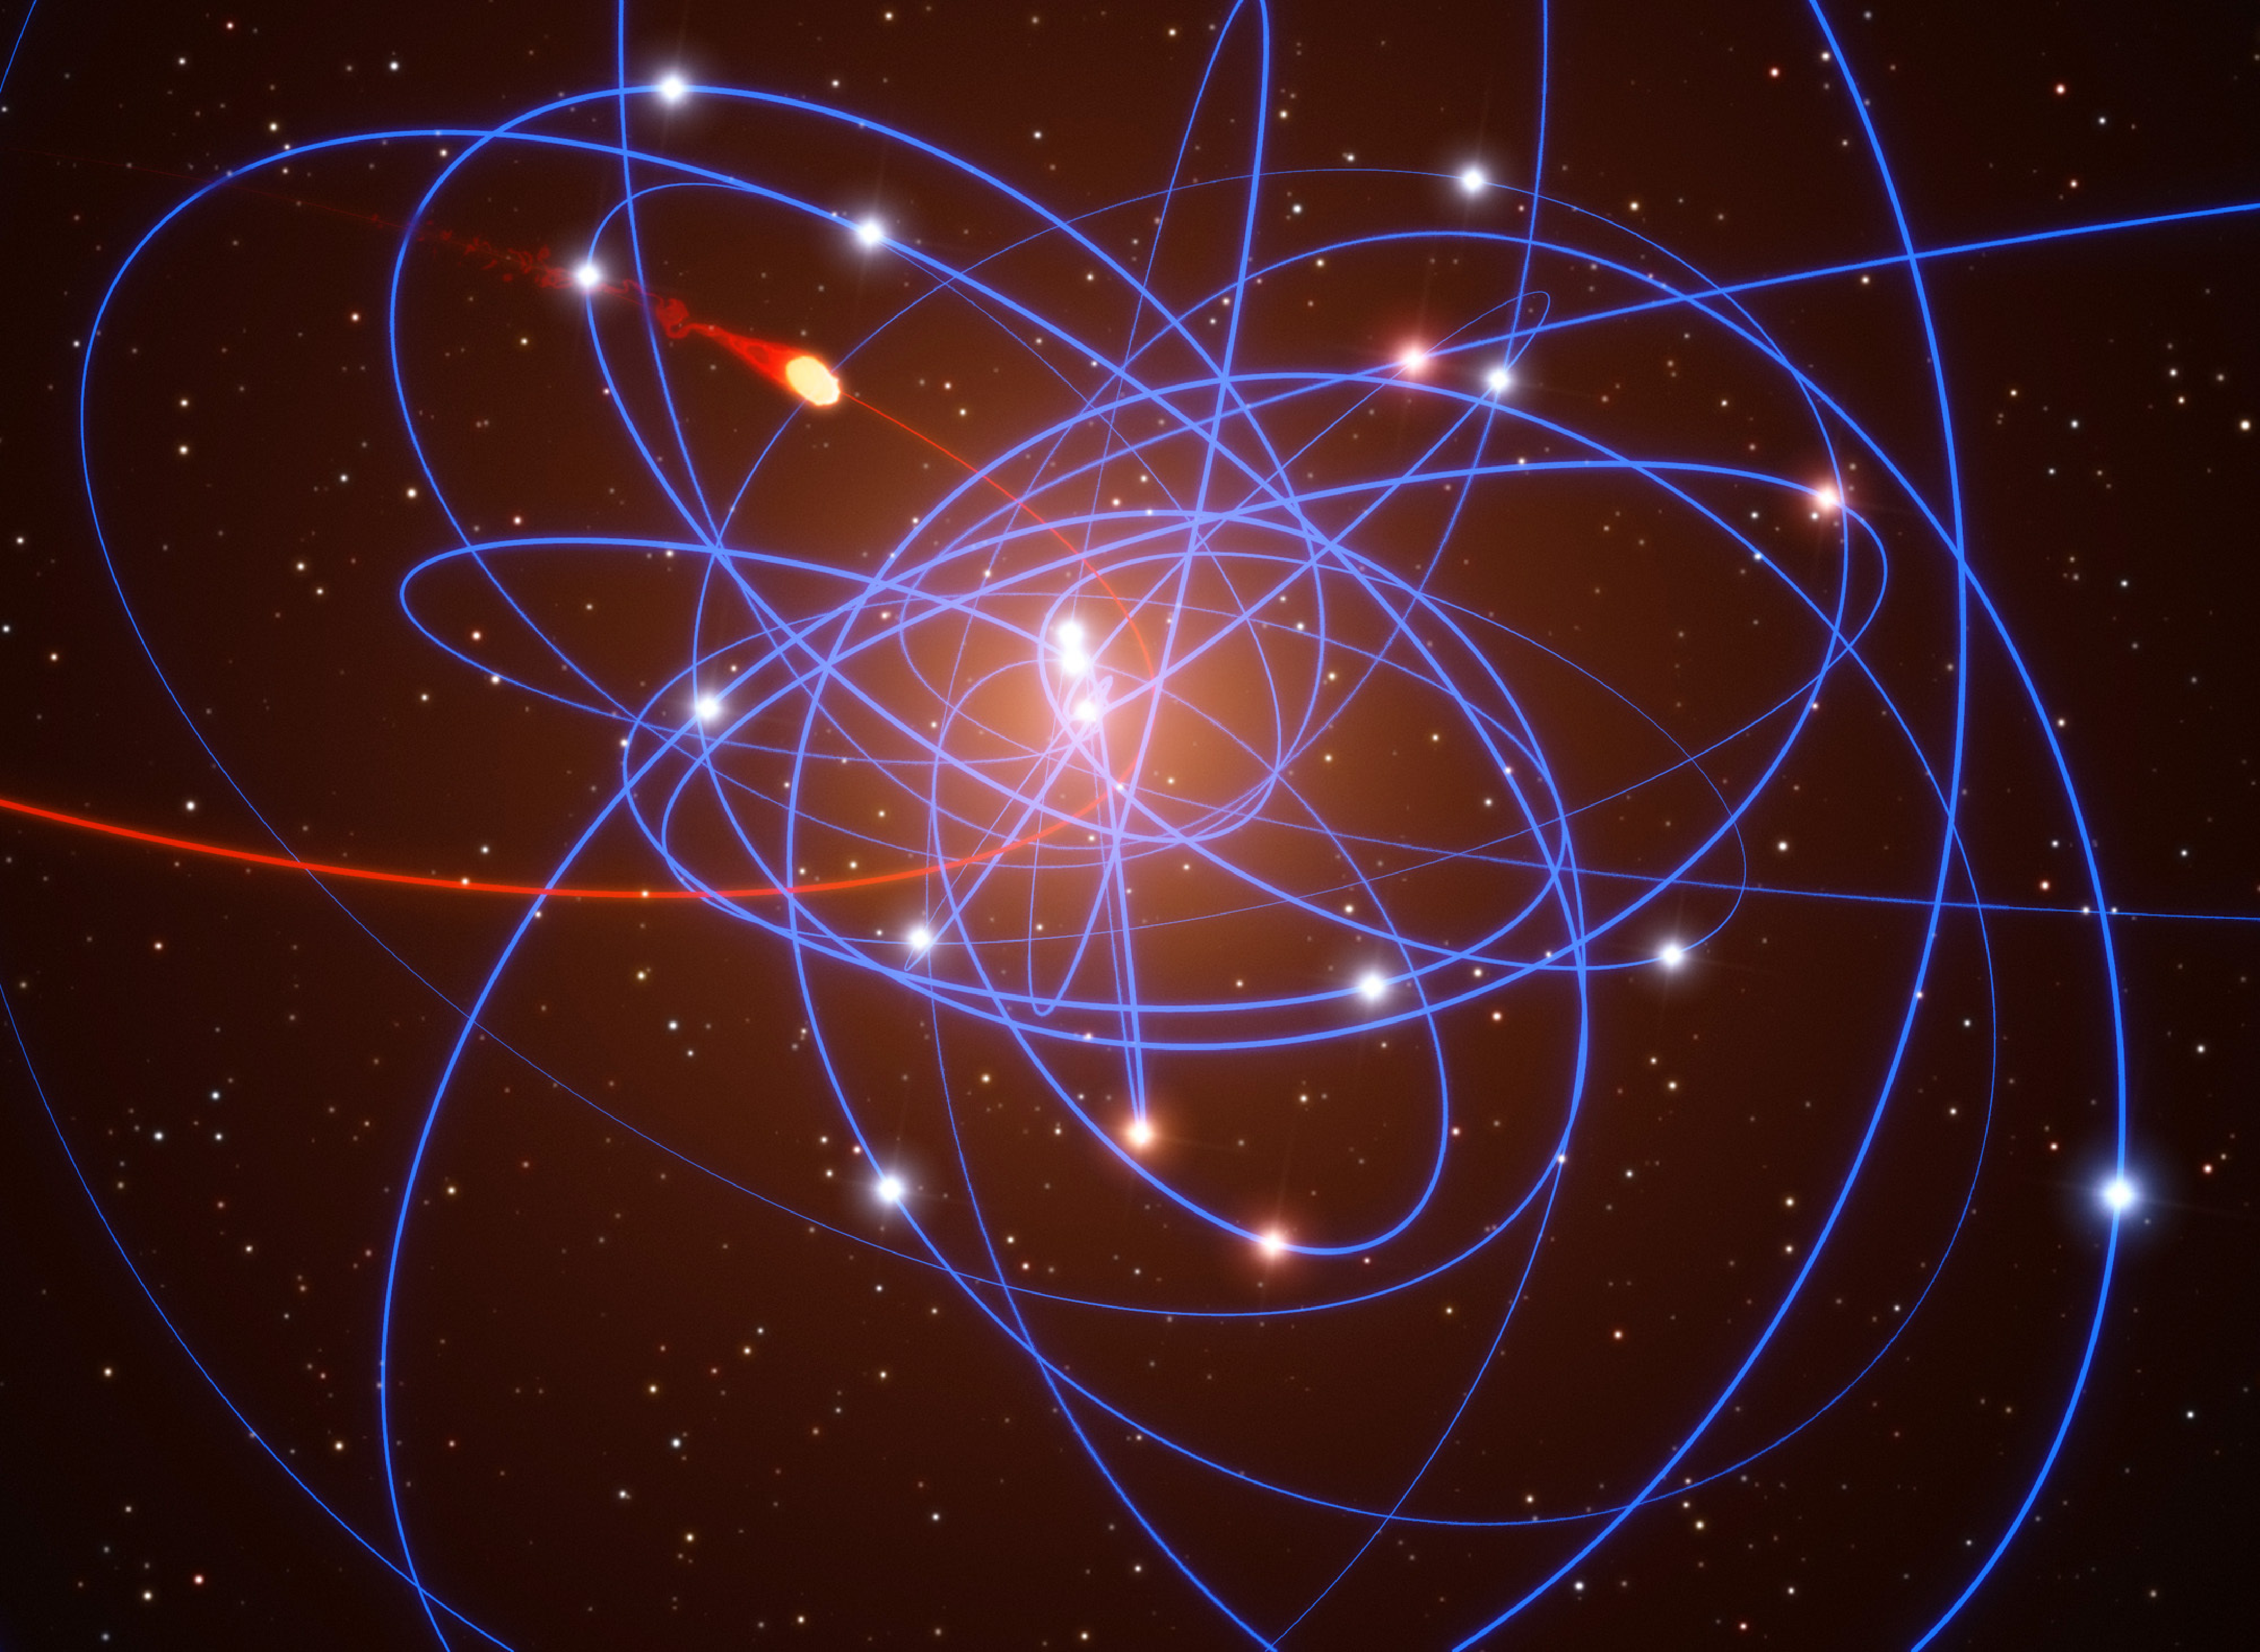
\includegraphics[width=\textwidth]{blackhole_MW_ESO.pdf}
%\end{wrapfigure}
%\end{center}
%\end{figure*}
\end{minipage}
}}
\end{figure*}



Looking at figure \ref{fig:rr} we see one radical difference in the shape of the effective potential with respect to the Newtonian case. At a certain critical radius $r=r_\mathrm{crit}$ the potential has a peak and thereafter it falls steeply downwards towards $r=0$. This is not surprising: Any particle which passes inside the horizon at $r=2M$ cannot escape. We see from figure \ref{fig:rr} that even objects with energies larger than $E/m=1$ (objects which are not bound in the classical sense) may be swallowed by the black hole. The objects with an energy $E/m$ larger than the critical energy $E_\mathrm{crit}/m$ will pass too close to the object, so close that $r<r_\mathrm{crit}$ and it is captured by the black hole. In the Newtonian case, this object would have a large enough energy to escape as $E/m>1$. In the exercises you will derive an expression for $E_\mathrm{crit}$. An object which enters the black hole with an energy $E=E_\mathrm{crit}$ equal the critical energy will make a few orbits around the black hole at $r=r_\mathrm{crit}$ before coincidences will make tiny changes to the energy of the object. These tiny changes may go in either direction, either the object will escape or the object will plunge into the black hole. We thus have three possibilities:
\begin{itemize}
\item $E/m<1$ which gives orbits
\item $1<E/m<E_\mathrm{crit}/m$ for which the object can move to infinity
\item $E/m>E_\mathrm{crit}/m$ for which the object will plunge into the black hole
\end{itemize}

There is one more important difference between the relativistic and the Newtonian effective potential. We will now consider a planet in orbit around a star. Because of the peak at $r=r_\mathrm{crit}$, the potential rises more steeply after the minimum than in the Newtonian case. A planet moving inwards in its orbit towards the star will thus have to climb up this steeper potential and will therefore slow down more close to the perihelion (the point in the orbit of a planet closest to the star). The radial velocity of the planet in the parts of the orbit close to the star is thus slower than in the Newtonian case. Since the planet then spends more time in the orbit close to the star, the planet now also has more time to move in the $\phi$ direction for which there is no slow-down. Thus, in general relativity the planet has moved more in the $\phi$ direction after passing close to the star than it would in the Newtonian case. How does this affect the orbit? The result is that the perihelion moves around the star. This is illustrated in figure \ref{fig:peripre}. For each orbit, the perihelion moves a little bit in $\phi$ direction. In Newtonian physics, the perihelion stays at the same point. This $\phi$ motion of the perihelion is called {\it perihelion precession}.

Long before Einstein discovered the general theory of relativity, it was well known that Mercury, the planet closest to the Sun, had a strong perihelion precession. A large part of this precession could be attributed to the gravitational forces from other planets in the solar system. But the gravitational attraction from other planets was not able to explain the full precession. A little part remained and it turned out that general relativity accounts for exactly this difference.

\section{Inside the horizon}

In the previous lecture we studied an object falling into the black hole from rest at a large distance from the black hole. We found that the conserved energy gave
\[
\sst\frac{dt}{d\tau}=1.
\]
Using this, we obtained the speed of the object as measured by the far-away observer
\[
\frac{dr}{dt}=-\sst\sqrt{\frac{2M}{r}}
\]
and the speed of the object measured by the local shell observers as the object passes the shells
\[
\frac{dr_\sh}{dt_\sh}=-\sqrt{\frac{2M}{r}}.
\]
What is the velocity $dr/d\tau$ measured on the wristwatch time $\tau$ of the falling object? Using these three equations we can write
\begin{align}
\label{eq:ff}
&\frac{dr}{d\tau}=\frac{dr}{dt}\frac{dt}{d\tau}=-\sst\sqrt{\frac{2M}{r}}\sst^{-1}\nonumber\\
&=-\sqrt{\frac{2M}{r}}.
\end{align}
Even when measuring velocity on the wristwatch of the object, the velocity approaches the speed of light at the horizon and gets larger than the speed of light inside the horizon. But who measures this velocity? Nobody! In this velocity measurement, length is measured by the far-away observer (who cannot measure anything after the object has entered the horizon) and time is measured on the wristwatch of the falling object. We also learned that inside the horizon there are no shell observers to measure the velocity since you cannot be at rest inside the horizon. A local observer sitting in an unpowered spaceship passing the object will always measure that the velocity is less than unity. Why? Because any freely falling observer is in a local inertial frame for a short moment when the spaceship passes nearby, even when inside the horizon. So for the freely falling observer special relativity applies (for a short moment when the spaceship passes nearby)) and he will always measure the velocity of the object as being less than the velocity of light.

How long will it take for the object to reach the singularity in the center from the moment it enters the horizon? We can integrate equation \ref{eq:ff} to find the time measured on the wristwatch of the object
\[
\tau=-\int_{2M}^0dr\sqrt{\frac{r}{2M}}=-\left[\frac{2}{3}\sqrt{\frac{r}{2M}}r\right]_{2M}^0=\frac{4M}{3}.
\]
How long will it take for an observer falling into a black hole with one solar mass to go from the horizon to the singularity? Measured on the wristwatch of the observer it takes
\begin{align*}
&\tau = \frac{4M_\odot}{3} =  \frac{4\times2\times10^{30}{\rm\ kg}\times7.42\times10^{-28}{\rm\ m/kg}}{3} \\
&\approx 2000{\rm\ m} \approx 7 {\rm\ \mu s}
\end{align*}

% \[
% \tau=\frac{4M_\odot}{3}=\frac{4\times2\times10^{30}{\rm\ kg}\times7.42\times10^{-28}{\rm\ m/kg}}{3}\approx2000{\rm\ m}=\frac{2000{\rm\ m}}{3\times10^8{\rm\ m/s}\approx7{\rm\ \mu s}.
% \]
In problem \refproblem{prob:insidehor}, you will study how the astronaut in a spaceship inside the horizon experiences the world.

\newpage
\pagestyle{headings}
%\TileWallPaper{51.5pt}{11.5pt}{noisy_grid.png}
\section{Exercises}

\newcounter{problem}
\newcommand{\newproblem}[1]{\refstepcounter{problem}\label{#1}{\bf Exercise \refproblem{#1}}}

\newproblem{prob:rocket}

Relevant theory: All sections.\newline
\begin{Figure}
\centering
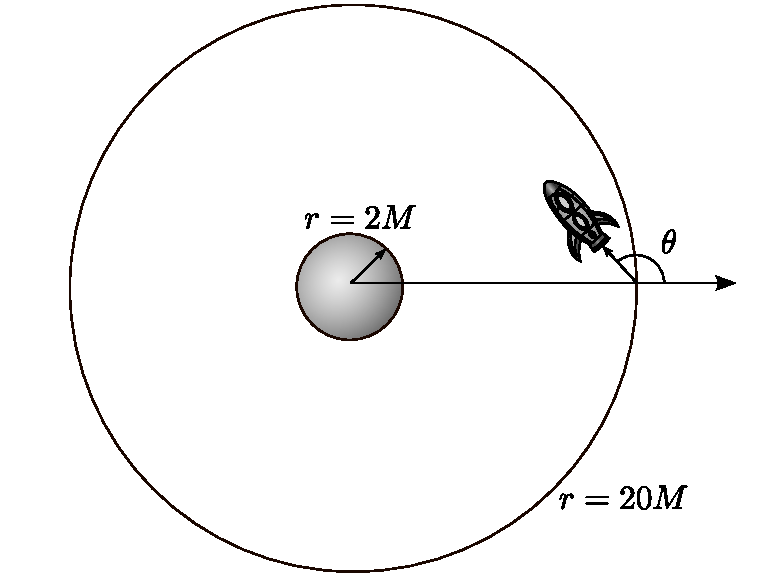
\includegraphics[width=\textwidth]{fig_17-9.pdf}
\captionof{figure}{Rocket launched from shell $r=20M$ inwards at an angle $\theta$. Note: Figure not to scale.\label{fig:rocket}}
\end{Figure}

A rocket is launched from shell at $R=20M$ around a black hole with mass $M$. The rocket has the velocity $v_\sh=0.993$ and is launched with $\theta=167^\circ$ where $\theta$ is defined as the angle from the radial vector to the velocity vector as seen in figure \ref{fig:rocket}. 

Just after launch the engines stop working. The astronaut therefore fear that his fate may lie within the black hole. In this exercise we will examine whether the rocket will be captured by the black hole or not. The rockets angular momentum is $L$ and the mass of the rocket is $m$. A relation that may come in handy is
\[
\frac{dx}{d\tau}=\frac{dx}{dt_\sh}\frac{dt_\sh}{d\tau},
\]
where $x$ can be any quantity.
\begin{enumerate}
\item Sketch a typical potential for a black hole. What criteria needs to be fulfilled to avoid crashing into the black hole?
\item We will now express the formula for the criteria in a more useful manner. Use the general relativistic expression for $E/m$ to show that the total energy per mass of the rocket can be written as
\[
\frac{E}{m}=\sqrt{1-\frac{2M}{R}}\gamma_\sh
\]
{\bf Hint:} Remember that for short time intervals $dt_\sh$, the shell observers can use special relativity. How would we write $dt/d\tau$ in special relativity?

\item Show that the angular momentum per mass for the rocket can be written as
\[
\frac{L}{m}=r^2\frac{d\phi}{d\tau}=R\gamma_\sh v_\sh \sin\theta,
\]
where $\gamma_\sh=1/\sqrt{1-v_\sh^2}$. \textbf{Hint:} A given relation may come in handy.

\item Use the general relativistic expression for the effective potential to show that the minimum and the maximum of the effective potential are located at the following distances(measured in \ss coordinates) from the black hole
\[
r_\mathrm{extremum}=\frac{(L/m)^2}{2M}\left(1\pm\sqrt{1-\frac{12M^2}{(L/m)^2}}\right).
\]
Use your earlier draft to determine which maximum corresponds to the leftmost peak? \textbf{Tips:} You are allowed to use an online calculator.

\item Insert numbers in the expression for $L/m$. Thereafter plot the potential for the rocket, mark the maximum effective potential and draw a horizontal line for the total energy per mass. Use the information from the drawing to tell if the rocket is captured by the black hole. \textbf{Use r in units of M.}

\item If he is captured by the black hole, how long does it take on the wristwatch of the astronauts to reach the singularity from the moment he enter the horizon. For simplicity ignore the angular momentum of the rocket $L/m=0$, use the black hole in the center of the Milky way with mass $M\approx4\times10^6M_\odot$ and give the answer in seconds.

{\bf Important hint:} In this exercise $E/M \neq 1$ and you can therefore not copy the result in the lecture note. Remember that you can use 'physics math' and exchange $\Delta$ with infinitesimals in an equation linking $\Delta r$ and $\Delta \tau$. For the integral, do yourself a favor and use an online calculator.

\item Now do the calculations numerically without ignoring the angular momentum. How important was the angular momentum L?

\item What will happen with the astronaut just before entering the singularity? Draw the gravitational forces on the astronaut (you can't really use forces but they are easier to draw and visualize than spacetime geometry). Which shape will he/she have just before reaching the center?
\end{enumerate}

\vspace{0.5cm}

\newproblem{prob:rocketorbit}

Relevant theory: All sections.\newline
In this exercise we will write a code to calculate the orbit of a spaceship around a black hole. For this we use polar coordinates and equation \ref{eq:phi} and \ref{eq:r}. We will use the program to simulate the trajectory of the spaceship from the previous exercise, therefore we will use the initial values given there.
\begin{enumerate}
\item Define variables for $(L/m)/M$ and $(E/m)$ by using the equations found in exercise 1 and the initial values given there. Define arrays for $r/M$ and $\phi$ with length $N=10000$ and the first element equal to their respective initial value, you can assume $\phi_0=0$ (this doesn't really matter for the final result, you can try changing it but keep it in radians).
\item Write two functions, one for equation \ref{eq:phi} and another for equation \ref{eq:r}.
\item Use Euler or Euler-Cromer to calculate the next values for $r/M$ and $\phi$ with $\Delta \tau=0.01$. Remember to check whenever the spaceship passes the Schwarzschild radius $r/M<2$ afterwards it cannot be seen (don't simulate for $r/M<2$).
\item Now plot the orbit and the Schwarzschild radius with the black hole at origin. You can here either transform from polar coordinates to Cartesian coordinates or use a useful function built into matplotlib.
\item How large angle $\Delta\phi$ did the spaceship revolve around the black hole before entering the horizon?
\end{enumerate}
Frode:

\vspace{0.5cm}

\newproblem{prob:insidehor}

Relevant theory: All sections.\newline
The rocket has entered the horizon and are falling towards the singularity, miraculously the engine starts working, is all hope truly lost or is there a way to escape. To study the possibility of escape the astronaut emits two light beams, one towards the central singularity and one backwards away from the singularity. 

In order to study how these beams of light are moving we need to write the \ss line element in terms of our wristwatch time $t'$ instead of \ss time $t$. We will make this change of coordinates already before entering the horizon as this allows us to use shell frames as a help. Assume in the following that we have velocity only in the radial direction. Assume also that we started falling freely with velocity $v=0$ far away from the black hole.
\begin{enumerate}
\item Use the Lorentz transformations to show that time intervals measured on the wristwatch of the astronaut are related to time and space intervals measured by shell observers as
\[
dt'=-v_\sh\gamma_\sh dr_\sh+\gamma_\sh dt_\sh,
\]
where $v_\sh$ and $\gamma_\sh$ are based on the local velocity of the astronaut measured by the shell observer at the shell which the spaceship passes. 
\item Use the expressions relating shell coordinates and \ss coordinates to show that
\[
dt'=-\frac{v_\sh\gamma_\sh dr}{\sqrt{\sst}}+\gamma_\sh\sqrt{\sst}dt.
\]
\item At the end of the lecture note we deduced the shell velocity $v_\sh$ of a falling spaceship starting with $v=0$ far from the black hole. Go back and check this expression. Insert it in the previous expression and show that
\[
dt=dt'-\frac{\sqrt{2M/r}dr}{\sst}.
\]
\item Use this to substitute $dt$ with $dt'$ in the normal \ss line element and show that the \ss line element can be written
\begin{align*}
&ds^2=d\tau^2=\\
&\sst(dt')^2-2\sqrt{\frac{2M}{r}}dt'dr-dr^2-r^2d\phi^2.
\end{align*}
Note that this form of the \ss line element does not have a singularity at $r=2M$.
\item We will now study the motion of the two light beams that we emit, one forwards and one backwards. We know that for light, proper time is not moving and $d\tau=0$. The light beams in this case are moving only radially so $d\phi=0$. Show that the speed of the two beams can be written as
\begin{equation} \label{eq:light_black_hole}
\frac{dr}{dt'}=-\sqrt{\frac{2M}{r}}\pm1.
\end{equation}
\item What is the physical interpretation of this equation, and more importantly can this speed be measured by any observers?
\item Based on equation \ref{eq:light_black_hole} how does the speed of the light beams change depending on the position of the rocket both outside and inside the horizon? What speed would the astronaut measure for the light beams?
\end{enumerate} 
We now have all the information needed to disclose whenever the astronaut have any possibilities to escape. So let's determine his/her fate by first studying the fate of the two emitted light beams.
\begin{enumerate}
\setcounter{enumi}{7}
\item Use equation \ref{eq:light_black_hole} to determine the direction of the emitted light beams inside the horizon.
\item The world line of the spaceship and the direction of the world lines for the two emitted light beams (arrows) has been plotted in figure \ref{fig:wl}. Use your previous results and equation \ref{eq:light_black_hole} to explain why the world lines for the light have the direction they have.
\item Looking at equation \ref{eq:light_black_hole} and figure \ref{fig:wl}, can the light beams exit the horizon?
\item By looking at the worldlines of light as well as the fact that light cannot escape the black hole. Does the astronaut with a rocket that can reach a velocity close to the speed of light escape the black hole?
\end{enumerate}


\begin{Figure}
\centering
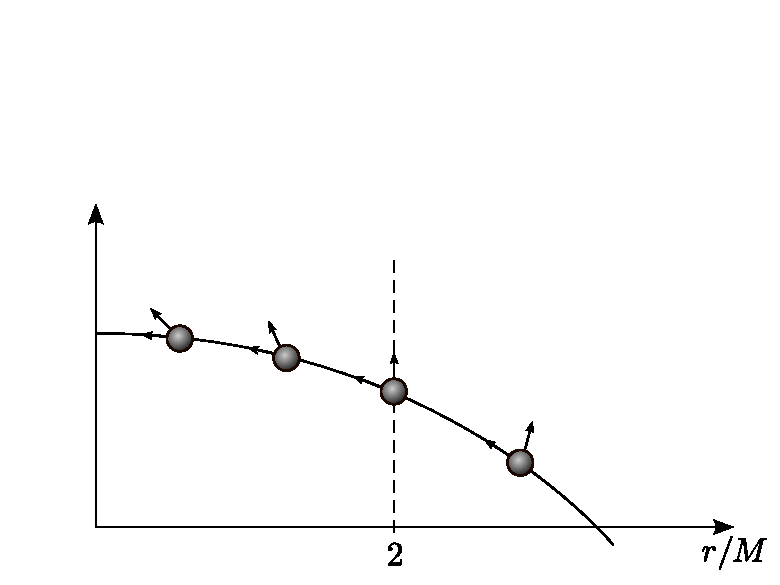
\includegraphics[width=\textwidth]{fig_17-10.pdf}
\captionof{figure}{Worldline of the rocket (marked by a balls) and parts of the worldlines of the forward and backward light beam (arrows) at several points during the free fall into the black hole.\label{fig:wl}}
\end{Figure}
\clearpage


\end{multicols}

\end{document}

